\chapter{モータ特性表自動生成ツール}\label{cha:Tool}
本章では、 本研究で試作したモータ特性表自動生成ツールについて説明する。
モータ特性表自動生成ツールは、モータのシミュレーション結果から、\ref{mortoku}節で述べたモータ特性表を自動生成する。
モータ特性表自動生成ツールの処理の流れを、図\ref{fig:kouzou}に示す。
\begin{figure}[t]
	\centering
	% \includegraphics[width=16.5cm]{./Image/.png}
	\includegraphics[width=14cm]{./Image/kouzou.png}
    \caption{モータ特性表自動生成ツールの構造}
	\label{fig:kouzou}
  \end{figure}
モータ特性表自動生成ツールの入力は、モータに関してシミュレーションしたOpenModelicaから出力されるcsvファイルである。ここで、現時点のツールは、実装上の都合により、入力となるcsvファイルは
次の3つの制約をすべて満たす必要がある。
\begin{itemize}
    \item モータのモデルがブラシ付きDCモータである
    \item モータの回路に印加する電圧値は一定
    \item 0秒からモータに入力を与える
\end{itemize}
モータ特性表自動生成ツールは、3つの処理部で構成しており、それぞれ以下の処理を行う。
\begin{itemize}
    \item csvファイル解析部
    \begin{itemize}
        \item 実行コマンドの取得
        \item csvファイルの読み込み
    \end{itemize}
    \item 特性表の要素算出部
    \begin{itemize}
        \item 基礎データの算出
        \item 特性表の構成要素の算出
    \end{itemize}
    \item モータ特性表生成部
    \begin{itemize}
        \item 特性表の生成
        \item 特性グラフの生成
        \item モータ特性表の生成
    \end{itemize}
\end{itemize}
以降、それぞれの処理部について説明する。
\section{csvファイル解析部}\label{csv_sec}
csvファイル解析部では、モータ特性表自動生成ツールを実行する際のコマンドから、読み込むcsvファイルを決定する。
そして、指定したcsvファイルを読み込み、モータ特性表を生成するために必要なデータを取得する。
以降、各処理について説明する。
\subsection{実行コマンドの取得}\label{sub:comand_get}
読み込むcsvファイルを特定するために、ツールを実行するコマンドの引数に、ファイル名を指定する。
モータ特性表自動生成ツールを実行するためのコマンドを、コード\ref{code:zikkou}に示す。
\begin{figure*}[t]
	\lstinputlisting[label={code:zikkou}, caption={実行コマンド}]{Image/comand.txt}
\end{figure*}
なお、このコマンドは、ツールの実行ファイルが存在するディレクトリで実行する必要がある。

第1引数には、入力とするcsvファイルのパスを含めたファイル名を指定する。

第2引数には、第1引数で指定したcsvファイルの中の、モータ特性表を自動生成したいモータのモデルに含まれる、慣性部品のオブジェクト名を指定する。

第3引数には、第1引数で指定したcsvファイルの中の、モータ特性表を自動生成したいモータのモデルに含まれる、電源部品のオブジェクト名を指定する。

第2引数と、第3引数に慣性部品と電源部品のオブジェクト名を指定する理由については、\ref{sub:csv_scan}節で述べる。

引数を取得するために、コマンドの引数を、1次元の配列で保持するsysライブラリのargvを使用する。
以下に、処理の流れを示す。

\begin{enumerate}
    \item argvの要素数を取得する
    \item 要素数が4以外であれば、図\ref{fig:error_hikisuu}のエラーを表示し、全体の処理を終了する
    \item argvの1番目の要素からファイル名を取得する
    \item 取得したファイル名の拡張子がcsvでない場合、図\ref{fig:error_file}のエラーを表示し、全体の処理を終了する
    \item argvの2番目の要素から慣性部品のオブジェクト名を取得する
    \item argvの3番目の要素から電源部品のオブジェクト名を取得する
\end{enumerate}

\begin{figure}[t]
	\centering
	\includegraphics[width=10cm,height=1.5cm]{./Image/error_tarinai.png}
	\caption{引数の数に誤りがあった場合のエラー文の例}
	\label{fig:error_hikisuu}
\end{figure}
\begin{figure}[t]
	\centering
	\includegraphics[width=12cm,height=1.5cm]{./Image/error_file.png}
	\caption{第1引数に誤りがあった場合のエラー文の例}
	\label{fig:error_file}
\end{figure}
\subsection{csvファイルの読み込み}\label{sub:csv_scan}
モータ特性表の要素を算出するために必要なデータを、csvファイルから取得する。
今回、モータ特性表の自動生成に必要となるデータの導出計算式は、以下の通りである。
% \vspace{3zh}
\begin{itemize}
    \item 効率
    \begin{eqnarray}
         \mbox{効率} = \frac{\mbox{出力}}{\mbox{入力}}  * 100 
        \end{eqnarray}

        \item 出力 
        \begin{eqnarray}
        \mbox{出力} = \mbox{トルク} * \mbox{角速度} 
         \end{eqnarray}
         
        \item 入力  \begin{eqnarray} \mbox{入力} = \mbox{電圧値} * \mbox{電流値} 
    \end{eqnarray}
        \item 回転数  \begin{eqnarray} \mbox{回転数} = \frac{30 * \mbox{角速度}}{\pi}   
    \end{eqnarray}
        \item 定格出力  \begin{eqnarray} \mbox{定格出力} = \mbox{定格トルク} * \mbox{定格回転数} * \frac{2\pi}{60} 
     \end{eqnarray}
     
\end{itemize}


上記の式より、モータ特性表の要素を算出するために必要なデータは、トルク、角速度、電圧、電流であると言える。
また、トルク、角速度、電圧、電流の値を持つcsvファイル内の変数を、表\ref{tab:hensuu}に示す。 
\begin{table}[t]
	\centering
	\caption{各値を持つ変数}
	\begin{tabular}{|c|c|} \hline
	  必要なデータ & 変数 \\ \hline \hline
	  トルク値 & (慣性部品のモジュール名).flange\_a.tau \\ \hline
	  角速度値 &  (慣性部品のモジュール名).w \\ \hline
	  電圧値 &  (電源部品のモジュール名).p.v \\ \hline
	  電流値 &  (電源部品のモジュール名).n.i \\ \hline
	\end{tabular}
	\label{tab:hensuu}
  \end{table}

モータ特性表自動生成ツールで、csvファイルを読み込むために、表\ref{tab:libr}で挙げたcsvライブラリを使用する。csvライブラリを用いた場合、csvファイルを1行ごとに分けて読み込む。
以下に、処理の流れを示す。
\begin{enumerate}
    \item csvファイルを読み込み専用で開く
    \item ファイルが開けなかった場合、図\ref{fig:error_file}のエラーを表示し、全体の処理を終了する
    \item csvファイルの行数分、以下の処理を繰り返す
    \begin{enumerate}
        \item csvファイルから取り出した行を、csvファイルの行の値を保持する配列rowに格納する。
        \item csvファイルの1行目を読み込んでいる場合、配列rowの要素数分、以下の処理を繰り返す
            \begin{enumerate}
                \item 変数名に、慣性部品のオブジェクト名が含まれている場合、以下の処理を行う
                \begin{enumerate}
                    \item 変数名の末尾に、「.flange\_a.tau」が含まれている場合、その変数名を格納している配列rowのインデックスを取得する
                    \item 変数名の末尾に、「.w」が含まれている場合、その変数名を格納している配列rowのインデックスを取得する
                \end{enumerate}
                \item 変数名に、電源部品のオブジェクト名が含まれている場合、以下の処理を行う
                \begin{enumerate}
                    \item 変数名の末尾に、「.p.v」が含まれている場合、その変数名を格納している配列rowのインデックスを取得する
                    \item 変数名の末尾に、「.n.i」が含まれている場合、その変数名を格納している配列rowのインデックスを取得する
                \end{enumerate}
            \end{enumerate}
            \item (a)で配列rowのインデックスを4つ取得するが、いずれか1つでも取得できない場合、図\ref{fig:error_comand}のエラーを表示し、全体の処理を終了する
    \end{enumerate}
        \item csvファイルの2行目を読み込んでいる場合、以下の処理を行う
        \begin{enumerate}
            \item 
        \end{enumerate}
        \item csvファイルの3行目以下を読み込んでいる場合、以下の処理を行う
        \begin{enumerate}
            \item トルク値を格納する配列である配列torqueに、3.(a).i.A.で取得した配列rowのインデックスにある値を格納する
            \item 角速度値を格納する配列である配列angularvelocityに、3.(a).i.B.で取得した配列rorwのインデックスにある値を格納する
            \item 電圧値を格納する配列である配列voltageに、3.(a).ii.A.で取得した配列rowのインデックスにある値を格納する
            \item 電流値を格納する配列である配列currentに、3.(a).ii.B.で取得した配列rowのインデックスにある値を格納する
        \end{enumerate}
\end{enumerate}
% なお、上記の処理の流れにおいて、
% csvファイルの2行目を読み込まない理由は、\ref{OM}節で述べたように、2行目にはモデルを作成した際の初期値が格納されており、初期値はモータ特性表の要素を算出することに使用しないからである。
\begin{figure}[t]
	\centering
	\includegraphics[width=12cm,height=1.5cm]{./Image/error_comand.png}
	\caption{第2引数、第3引数に誤りがあった場合のエラー文の例}
	\label{fig:error_comand}
\end{figure}
\section{特性表の要素算出部}\label{youso_sec}
特性表の要素算出部では、\ref{csv_sec}節で取得したデータをもとに、特性表の各要素を算出する。
まず、特性表の各要素を算出するために必要となる基礎データを算出する。基礎データとは、回転数、出力、効率の値のことを指す。
そして、\ref{csv_sec}節で取得したデータと基礎データから特性表の各要素を算出する。
以降、各処理について説明する。
\subsection{基礎データの算出}\label{sub:youso_kiso}
基礎データの算出処理では、回転数、出力、効率の値を持つ配列を、それぞれの値に対して生成する。
生成方法を以下に示す。
\subsubsection{回転数}\label{sub:sub:kaiten}
% 回転数を算出する式は、\ref{sub:csv_scan}節の箇条書き中にある、回転数にて示した式を用いる。
回転数を算出する式は、\ref{sub:csv_scan}節の(3.4)式を用いる。
配列angularvelocityから、配列の要素数分、繰り返し処理で、回転数の値を持つ配列speedを生成する。
\subsubsection{出力}\label{sub:sub:syutu}
% 出力を算出する式は、\ref{sub:csv_scan}節の箇条書き中にある、出力にて示した式を用いる。
出力を算出する式は、\ref{sub:csv_scan}節の(3.2)式を用いる。
配列torqueと、配列angularvelocityから、配列の要素数分、繰り返し処理で、出力の値を持つ配列outputを生成する。
\subsubsection{効率}\label{sub:sub:kouritu}
% 効率を算出する式は、\ref{sub:csv_scan}節の箇条書き中にある、効率にて示した式と入力にて示した式を用いる。
効率を算出する式は、\ref{sub:csv_scan}節の(3.1)式と、(3.3)式を用いる。
まず、配列voltageと、配列currentから、(3.3)式を用いて入力値を求める。
そして、配列outputと、求めた入力値から、配列の要素数分、繰り返し処理で、効率の値を持つ配列efficiencyを生成する。
\subsection{特性表の各要素の算出}\label{sub:youso_mortoku}
特性表の各要素の算出処理では、\ref{sub:tokuseihyou}節で述べた9つの要素を算出する。
それぞれの算出方法を以下に示す。
\subsubsection{電圧}\label{sub:sub:dennatu}
モータ特性表自動生成ツールが対応するモデルでは、電圧値が一定のため、配列voltageの要素はすべて同じ値になる。今回は、0番目の値を電圧とする。
\subsubsection{始動電流}\label{sub:sub:sidouden}
始動電流とは、モータの起動時に流れる大きな電流であり、モータが起動した後は逆起電力が発生するため、モータ・コイル部分にかかる電圧が下がり、電流値も下がる。
したがって、配列currentの要素の最大値を始動電流とする。
\subsubsection{停動トルク}\label{sub:sub:teidoutoruku}
停動トルクとは、モータが出しうる最大のトルク値である。したがって、配列torqueの最大値を停動トルクとする。
\subsubsection{最大効率}\label{sub:sub:saidaikouritu}
配列efficiencyの最大値を最大効率とする。
\subsubsection{定格トルク}\label{sub:sub:teikakutoruku}
定格トルクとは、最大効率時のトルク値である。まず、配列efficiencyの中で、最大効率である要素のインデックスを取得する。
そして、配列torqueの中で、取得した最大効率のインデックスと同じ位置にある値を定格トルクとする。
\subsubsection{定格回転数}\label{sub:sub:teikakukaiten}
定格回転数とは、最大効率時の回転数の値である。配列speedの中で、取得した最大効率のインデックスと、同じ位置にある値を定格回転数とする。
\subsubsection{定格電流}\label{sub:sub:teikakuden}
定格電流とは、最大効率時の電流値である。配列currentの中で、取得した最大効率のインデックスと、同じ位置にある値を定格電流とする。
\subsubsection{定格出力}\label{sub:sub:teikakusyutu}
定格出力とは、定格動作点における出力の値である。定格出力を算出する式は、\ref{sub:csv_scan}節の(3.5)式を用いる。
上記の定格トルクと定格回転数で求めた値を、定格出力を算出する式に代入し、得た値が定格出力である。
\subsubsection{最大回転数}\label{sub:sub:saidaikai}
最大回転数とは、配列speedの最大値を最大回転数とする。
\section{モータ特性表生成部}\label{mortoku_sec}
モータ特性表生成部では、\ref{csv_sec}節と\ref{youso_sec}節で算出した要素を用いて、モータ特性表を自動生成する。まず、特性表を生成し、画像として保存する。
次に、\ref{sub:tokuseigurahu}節で挙げた4つの特性グラフを生成し、画像として保存する。最後に、特性表の画像と、特性グラフの画像をPDFファイルに書き込むことで、モータ特性表を自動生成する。
以降、各処理について説明する。
\subsection{特性表生成}\label{sub:mortortoku}
この処理では、\ref{sub:youso_mortoku}節で作成した特性表の要素の配列を用いて、特性表を生成する。処理の流れを以下に示す。
\begin{enumerate}
    \item 特性表の各要素の名前を持つ配列を作成する(コード\ref{code:name}参照)
    \item 特性表の要素の配列と、特性表の各要素の名前を持つ配列から、特性表用の配列を作成する
    \item 特性表用の配列から特性表を生成し、生成した表の上部に「モータ特性表」の文字を追加し、画像として保存する。
\end{enumerate}
上記の処理で生成した特性表の画像を、図\ref{fig:toku_gazou}に示す。
\begin{figure*}[t]
	\lstinputlisting[label={code:name}, caption={特性表を構成する要素名の配列}]{Image/name.txt}
\end{figure*}
\begin{figure}[t]
	\centering
	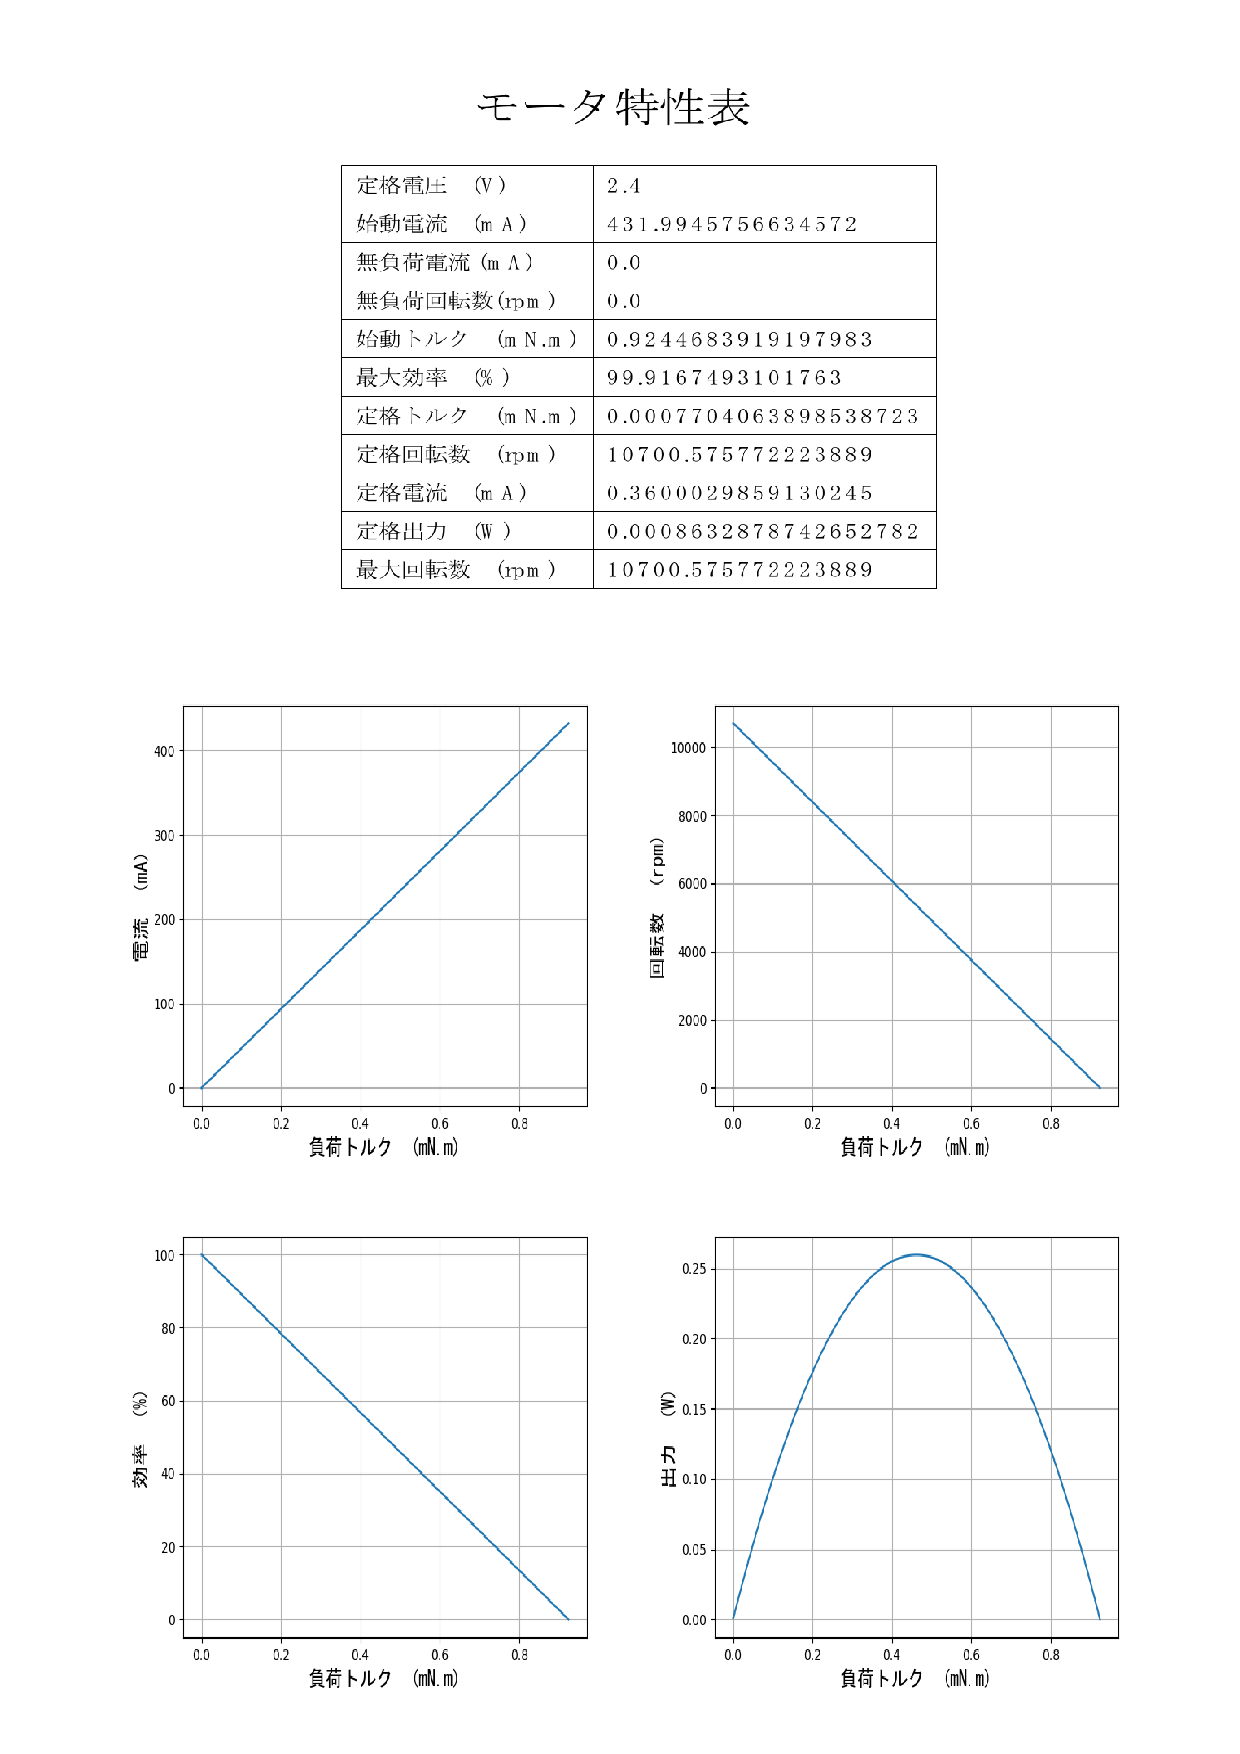
\includegraphics[width=7cm]{./Image/characteristicTable.png}
	\caption{特性表の画像}
	\label{fig:toku_gazou}
\end{figure}
\subsection{特性グラフ生成}\label{sub:toku_gurahu}
\ref{sub:csv_scan}節、\ref{sub:youso_kiso}節で求めた要素の配列を用いて、特性グラフを生成する。
処理の流れを以下に示す。
\begin{enumerate}
    \item x軸にトルク値を持つ配列を、y軸に電流値を持つ配列を指定してグラフを生成し、画像として保存する
    \item x軸にトルク値を持つ配列を、y軸に回転数値を持つ配列を指定してグラフを生成し、画像として保存する
    \item x軸にトルク値を持つ配列を、y軸に効率値を持つ配列を指定してグラフを生成し、画像として保存する
    \item x軸にトルク値を持つ配列を、y軸に出力値を持つ配列を指定してグラフを生成し、画像として保存する
\end{enumerate}
上記の処理で生成した4つのグラフを、それぞれ図\ref{fig:current}、図\ref{fig:speed}、図\ref{fig:effi}、図\ref{fig:output}に示す。
\begin{figure}[t]
	\centering
	\includegraphics[width=7cm]{./Image/current.png}
	\caption{「トルク * 電流」グラフ}
	\label{fig:current}
\end{figure}
\begin{figure}[t]
	\centering
	\includegraphics[width=7cm]{./Image/speed.png}
	\caption{トルク * 回転数」グラフ}
	\label{fig:speed}
\end{figure}
\begin{figure}[t]
	\centering
	\includegraphics[width=7cm]{./Image/efficiency.png}
	\caption{「トルク * 効率」グラフ}
	\label{fig:effi}
\end{figure}
\begin{figure}[t]
	\centering
	\includegraphics[width=7cm]{./Image/output.png}
	\caption{「トルク * 出力」グラフ}
	\label{fig:output}
\end{figure}
\subsection{モータ特性表生成}\label{sub:}
\ref{sub:mortortoku}節と、\ref{sub:toku_gurahu}節で生成した合計5つの画像を、PDFファイルに書き込み、モータ特性表を自動生成する。
モータ特性表のPDFファイルのファイル名は、「characteristicTable.pdf」で生成する。同じファイル名がある場合、上書き保存する。
この処理で自動生成するモータ特性表を、図\ref{fig:tokuseihyou}に示す。
\begin{figure}[t]
	\centering
	\fbox{
	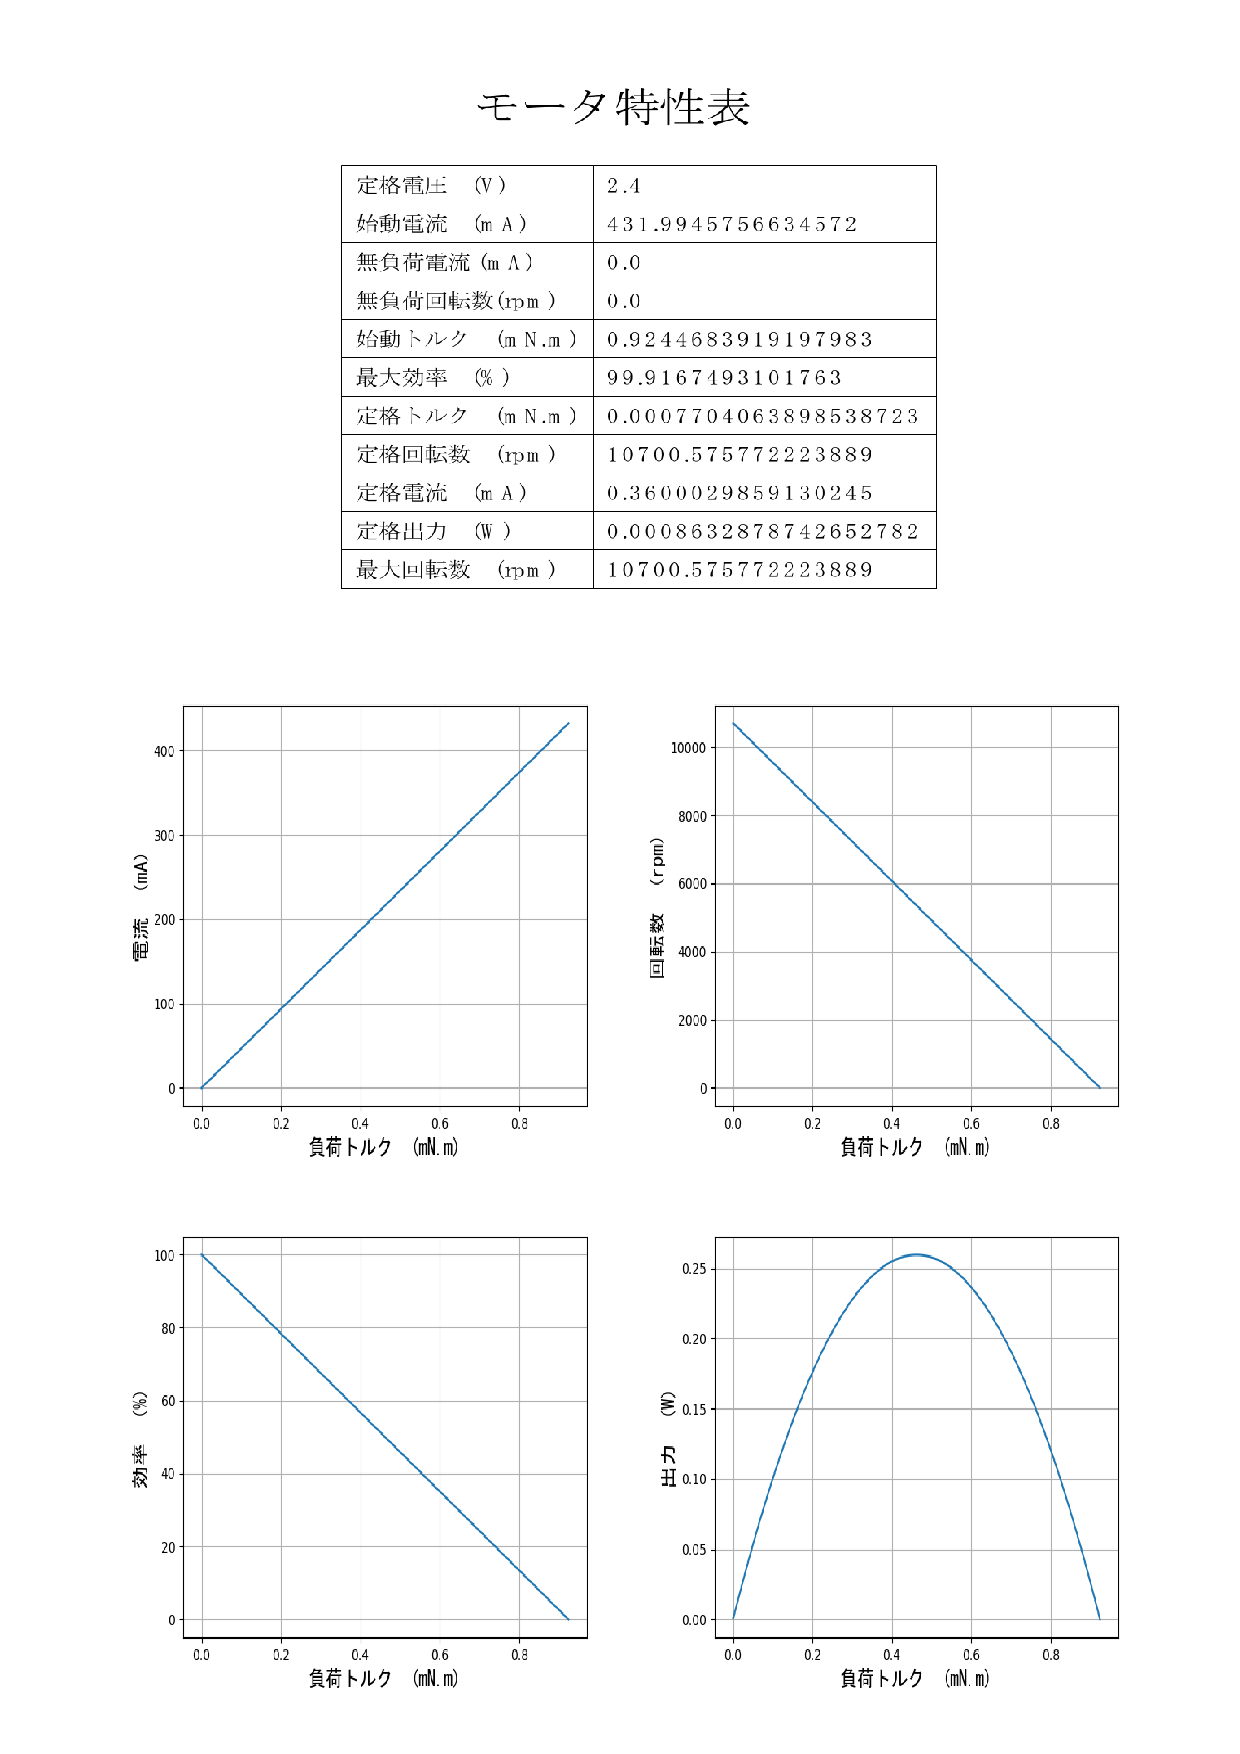
\includegraphics[width=16cm,pagebox=cropbox]{Image/characteristicTable.pdf} 
	}
	\caption{モータ特性表}
	\label{fig:tokuseihyou}
\end{figure}